\section{AL}\label{sec:al}

This section explains about syntax and semantics of AL.
\footnote{Note that this is NOT a syntax and semantics of WebAssembly, but rather,
syntax and semantics of prose notation of WebAssembly Specification}

\subsection{Syntax}

This section describes the syntax of AL.

\begin{minipage}{0.5\textwidth}
$$
\begin{array}{@{}lrrl@{}}
\text{Specification} & \mathsf{s} &::=& {\mathsf{A}^\ast} \\
\text{Algorithm} & \mathsf{A} &::=& \mathsf{algorithm}~\mathit{f}~({\mathit{e}^\ast})~\{{\mathsf{i}^\ast}\} \\
\text{Instruction} & \mathsf{i} &::=& \mathsf{if}~\mathit{c}~{\mathsf{i}^\ast}~{\mathsf{i}^\ast}^? \\ &&|&
\mathsf{either}~{\mathsf{i}^\ast}~{\mathsf{i}^\ast} \\ &&|&
\mathsf{enter}~{\mathsf{e}}~{\mathsf{e}}~{\mathsf{i}^\ast} \\ &&|&
\mathsf{assert}~\mathit{c} \\ &&|&
\mathsf{push}~\mathit{e} \\ &&|&
\mathsf{pop}~\mathit{e} \\ &&|&
\mathsf{popall}~\mathit{e}~\mathit{c} \\ &&|&
\mathsf{let}~\mathit{e}~\mathit{e} \\ &&|&
\mathsf{trap} \\ &&|&
\mathsf{nop} \\ &&|&
\mathsf{return}~{\mathit{e}^?} \\ &&|&
\mathsf{execute}~\mathit{e} \\ &&|&
\mathsf{executeall}~\mathit{e} \\ &&|&
\mathsf{perform}~\mathit{e} \\ &&|&
\mathsf{exit} \\ &&|&
\mathsf{ref}~\mathit{x}~\mathit{e} \\ &&|&
\mathsf{replace}~\mathit{e}~\mathit{p}~\mathit{e} \\
\text{Condition} & \mathit{c} &::=& \sim\mathit{c} \\ &&|&
\mathit{c}(\wedge)\mathit{c} \\ &&|&
\mathit{e}(<)\mathit{e} \\ &&|&
\mathit{e}<:\mathit{s} \\ &&|&
\mathsf{valid}~\mathit{e} \\
\end{array}
$$
\end{minipage}
\begin{minipage}{0.5\textwidth}
$$
\begin{array}{@{}lrrl@{}}
\text{Expression} & \mathit{e} &::=& \mathit{n} \\ &&|&
\mathit{s} \\ &&|&
\mathit{op}(\mathit{e^\ast}) \\ &&|&
\mathit{e}^\ast \\ &&|&
\mathit{e}^\mathit{e} \\ &&|&
\mathit{e}^? \\ &&|&
\mathit{e}::\mathit{e} \\ &&|&
|\mathit{e}| \\ &&|&
\{{(\mathit{s} \rightarrow \mathit{e})^\ast}\} \\ &&|&
\mathit{e}[\mathit{p}] \\ &&|&
\mathit{e}[\mathit{p}^\ast:+=\mathit{e}] \\ &&|&
\mathit{e}[\mathit{p}^\ast:=\mathit{e}] \\ &&|&
\mathit{s}(\mathit{e}^\ast) \\ &&|&
(\mathit{e},\mathit{e}) \\ &&|&
\mathit{x} \\ &&|&
\mathit{e}^{\{\mathit{x}^\ast\}~\mathit{iter}} \\
\text{Iter} & \mathit{iter} &::=& \mathsf{?} \\ &&|&
\mathsf{\ast} \\ &&|&
\mathsf{+} \\ &&|&
{(\mathit{x}<)}^?~\mathit{e} \\
\text{Path} & \mathit{p} &::=& [\mathit{e}] \\ &&|&
[\mathit{e}:\mathit{e}] \\ &&|&
.\mathit{s} \\
\text{Program} & \mathit{n} &\in& \mathbb{N} \\
\text{String} & \mathit{s} &\in& \mathit{Id} \\
\text{Variable name} & \mathit{x} &\in& \mathit{Id} \\
\text{Function name} & \mathit{f} &\in& \mathit{Id} \\
\end{array}
$$
\end{minipage}

Metavariable
$\mathsf{p}$ ranges over a program,
$\mathsf{A}$ ranges over an algorithm,
$\mathsf{i}$ ranges over an instruction,
$\mathit{c}$ ranges over a condition,
$\mathit{e}$ ranges over an expression,
$\mathit{iter}$ ranges over an iter-expression,
$\mathit{p}$ ranges over a path,
$\mathit{n}$ ranges over an integer,
$\mathit{s}$ ranges over a string,
$\mathit{x}$ ranges over a variable name.
and
$\mathit{f}$ ranges over a function name.

An AL program $\mathsf{p}$ consists of algorithms $\mathsf{A}^\ast$.  An
algorithm $\mathsf{A}$ has its name $\mathit{f}$, parameters
${\mathit{e}^\ast}$, and its body instructions ${\mathit{i}^\ast}$.  There are
various types of instructions including familiar push/pop instructions. The
instructions are designed in a way that it resembles the prose statements
appearing in the official specification.  For example, the prose `2. Pop the
value val from the stack` in Fig~\ref{fig:prosespec1} corresponds to the following
instruction: $\mathsf{pop} \mathit{val}$. Various kinds of conditions and expressions are
are also designed to closely reflect the prose appearing in the specification.
The detailed role of each instructions, conditions, and expressions will be discussed
in the semantics section.

\subsection{Semantics}

This section describes the semantics of AL.
The execution of a programs starts by calling an AL algorithm,
which sequentially executes its body instruction.
The semantics of AL is defined in terms of \textit{state} transition.
Executing one AL instruction alters the program state,
and the final state after executing the last instruction of an algorithm is the
final result of the program execution. 

\begin{figure}
  \centering
  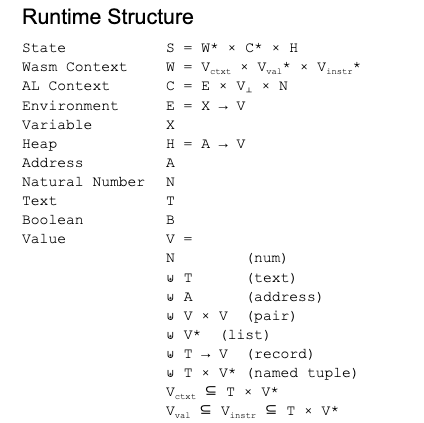
\includegraphics[width=0.5\textwidth]{img/runtime.png}
  \caption{Runtime structure}
  \label{fig:runtime}
\end{figure}

Figure~\ref{fig:runtime} describes the runtime structure of AL, including the state.
A state is a triplet of three elements: a stack of Wasm contexts, a stack of AL contexts, and a heap.

The role of a Wasm context is to keep track of Wasm's control flow. For example,
the semantics of Wasm instructions that change the control flow of Wasm, such as `Call` or `Return`,
is described using the prose
`11. Enter the instruction sequence instr* with label L` or
`10. Jump to the instruction after the original call that pushed the frame`.
When executing the AL instructions that corresponds to these prose, then a Wasm context is
pushed or popped to the Wasm context of the current state.
A Wasm context is a triplet of three elements: a value denoting the context kind, a stack of Wasm values,
and a stack of Wasm instructions. The context kind and additional information of the context.
The current version of Wasm specification has two kinds of context kinds: label and frame.
When the additional features like exception handling are added to Wasm, new contexts such as
'handler' or 'caught' may be introduced, which also can be handled generally.
The Wasm value stack is the stack to keep the pushed Wasm values. This stack is the one that is
modified by the AL `pop` or `push` instructions. The Wasm instruction stack keeps the list of
next Wasm instructions to be executed. When the current Wasm instruction is finished, then
the next Wasm instruction which is on the top of Wasm instruction stack will be handled.
Overall, the Wasm context is altered by executing Wasm-specific AL instructions,
such as enter, exit, push or pop.

The role of AL context is to keep track of AL's control flow; more specifically, the calling context.
Whenever a new AL algorithm is called, a new AL context is pushed to the stack, and returning from
an algorithm pops a context form the stack. An AL stack is a triplet of three elements:
the environment, the return value, and an integer for Wasm context counter.
The environment is a typical mapping from the variable to the values. The return value is
indicates the return value of the current algorithm. It is initially bottom when an algorithm starts,
and if an AL return instruction is executed, the return value is set to that value an rest of
AL instructions are skipped. The Wasm context counter is a bit tricky one. It's goal is to
keep track of how many Wasm contexts were created within this AL context. This number is
needed to concisely describe the correct behavior of `enter` and `exit`.

The heap is a typical mapping from the addresses to the values. Heap enables the mutation
in an AL program, such as `replace` instruction.

An AL value v is either a number n, a text t, an address a, a tuple (v1, v2),
a list v*, a record (t -> v), or a named tuple (t, v*). The value that denotes
the Wasm context kind is a subset of named tuples. Note that the Wasm values (i.e. i32.const 42) are
subset of Wasm instructions, which are both encoded as named tuple values in AL.

\begin{figure}
  \centering
  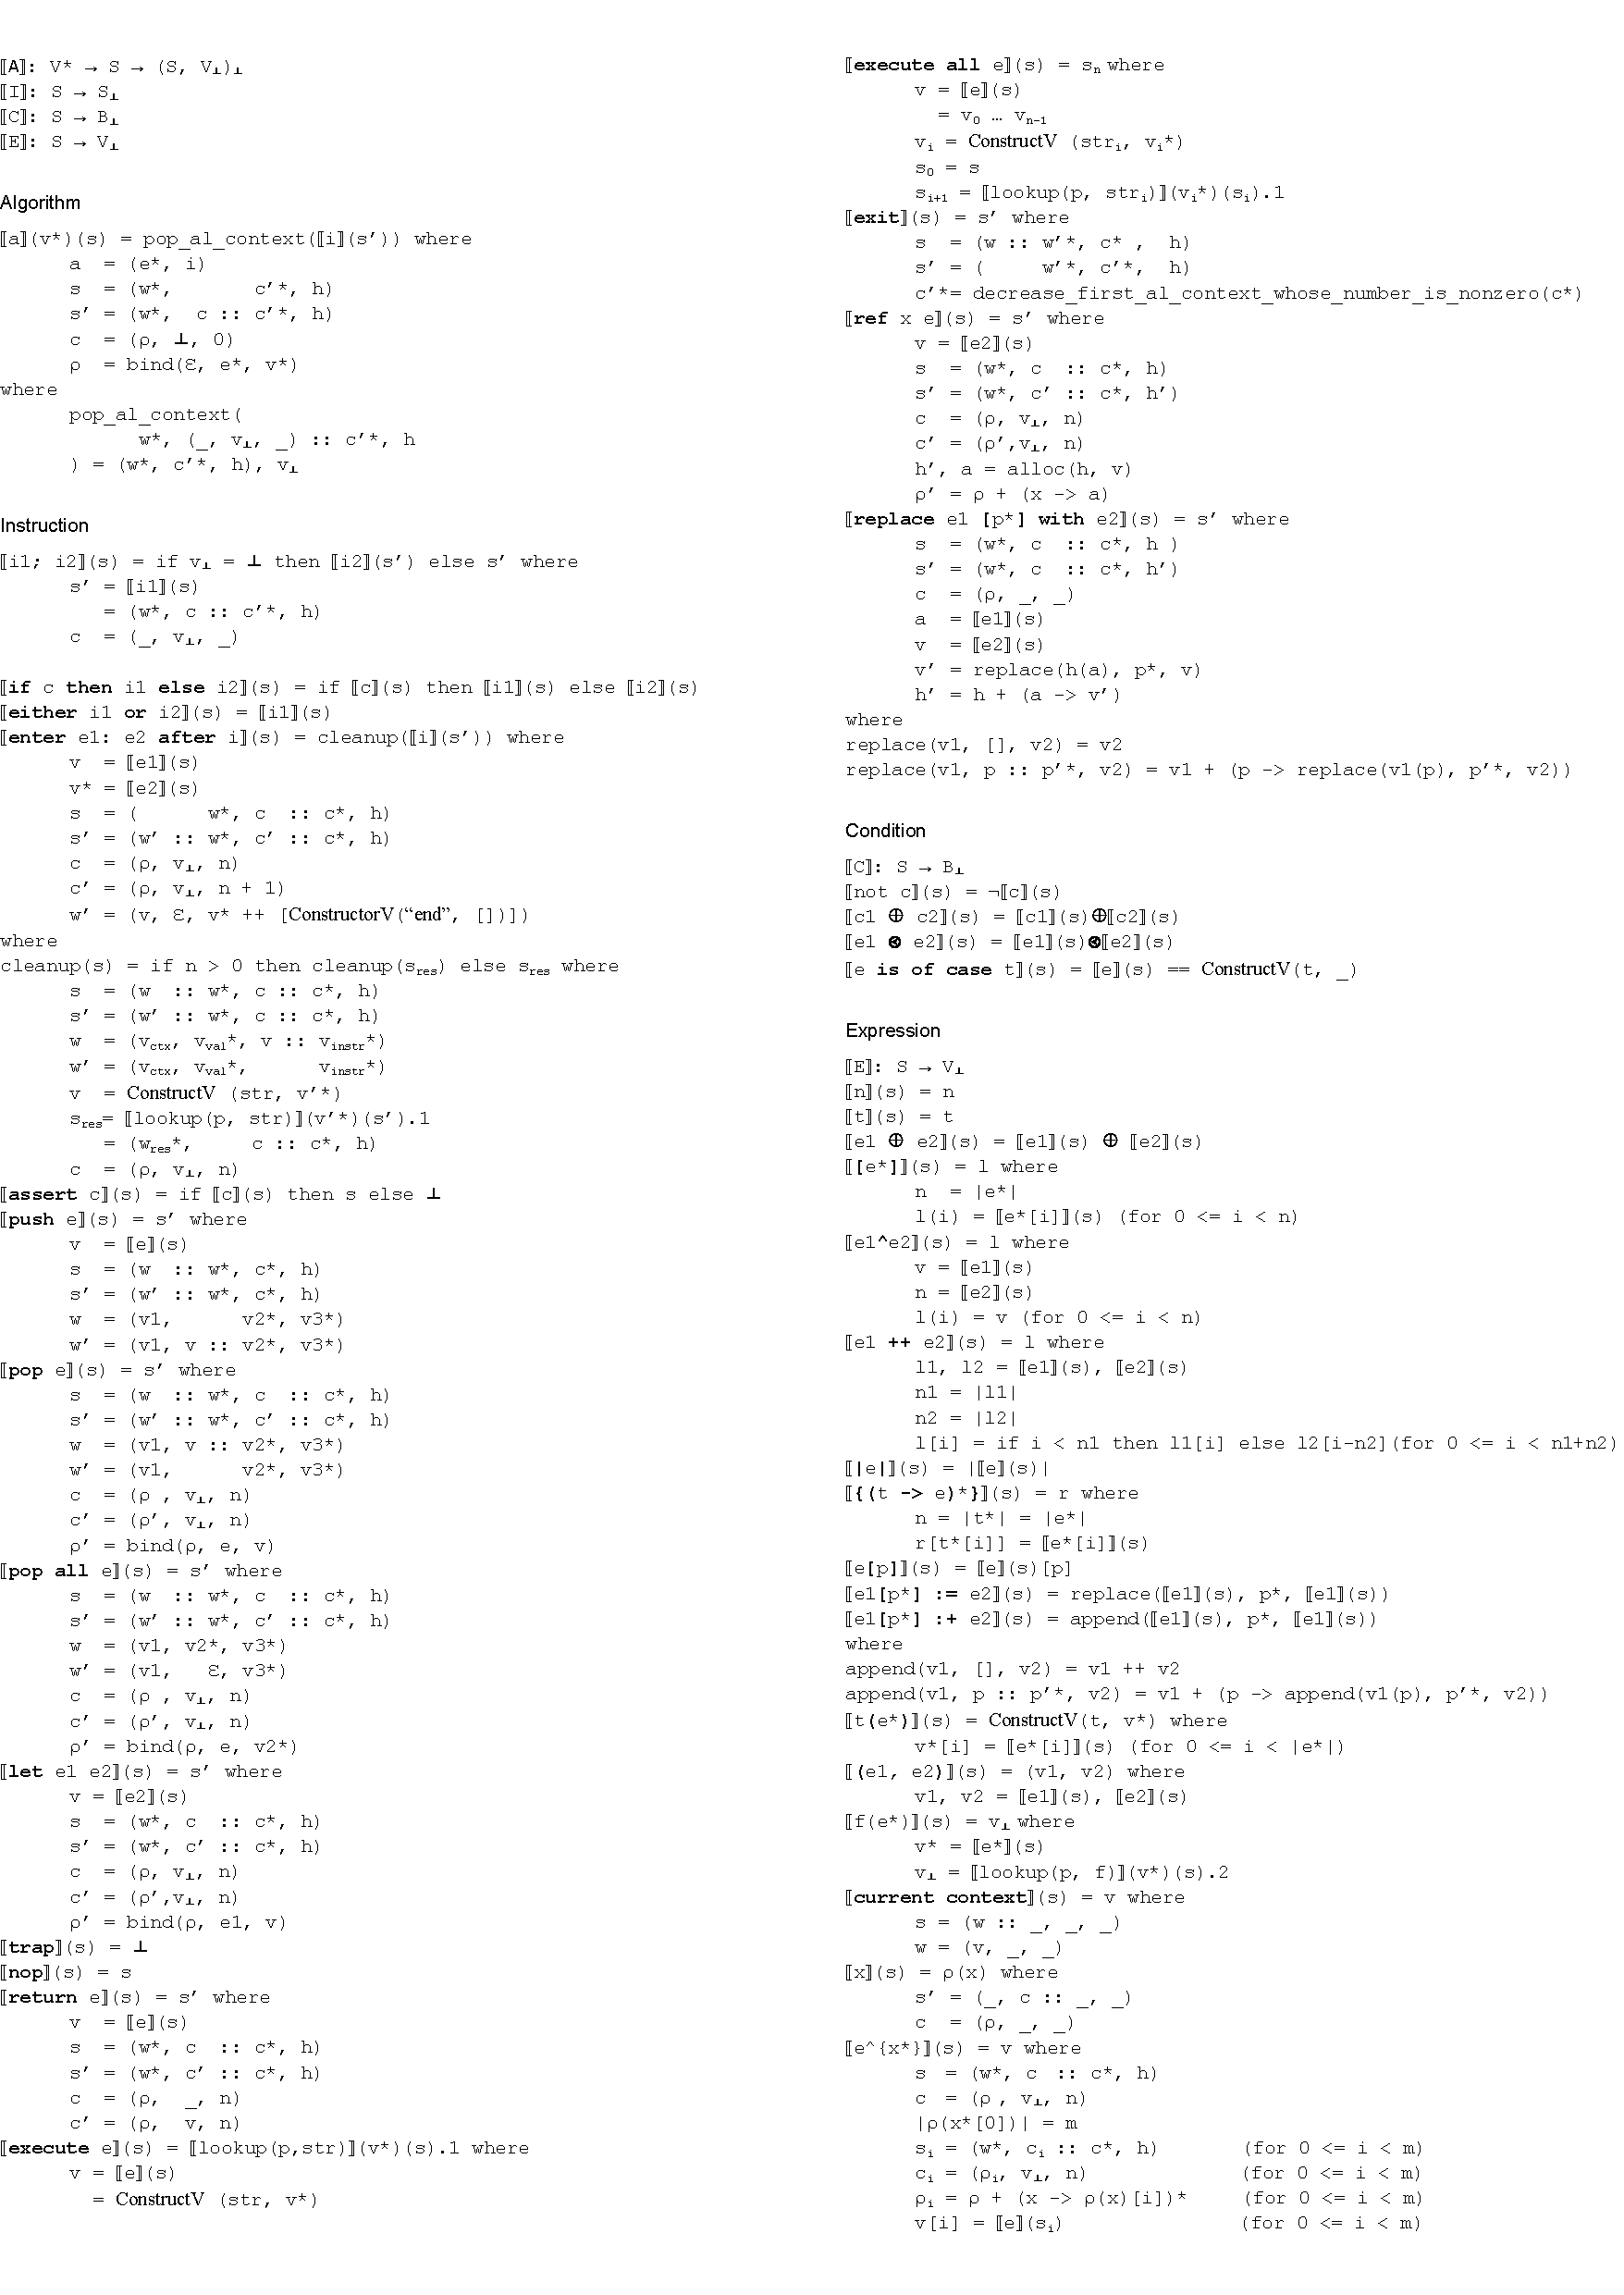
\includegraphics[width=\textwidth]{img/Semantics.pdf}
  \caption{Semantics}
  \label{fig:semantics}
\end{figure}

Figure~\ref{fig:semantics} illustrates the denotational semantics of executing an AL algorithms, instructions,
conditions and expressions. The function signatures in first four lines
indicate the input and output of the execution for each component.
Argument values and a state is given as an input for executing an algorithm,
and the new state after executing the algorithm and the return value of the algorithm (if exits) is returned.
A state is given as an input for executing an instruction,
and the new state after executing the instruction is returned.
A state is given as an input for evaluating a condition, and the boolean value is returned.
Finally, A state is given as an input for evaluating an expression, and the value is returned.
Note that evaluating a condition or an expression is pure: there is no modification in state.
Also, the execution or evaluation may incur a runtime error, (i.e. executing Trap AL instruction
/ out of boundary access), which is indicated by the fact that the range of each function
is lifted with the bottom ($\bot$) element.

An algorithm a = (e*, i) is executed by executing its body instruction i under a newly created context c.
The new context c consists of the initial environment $\rho$, unset return value $\bot$ and a
Wasm context counter value 0. The initial environment $\rho$ is initialized by binding
each given argument to each parameter. The helper function `bind` handles the
destructuring binding, where the lhs of binding is a complex pattern, not a single variable.
For example, to handle the destructuring binding of the form `Let (a,b) = (1,2)`,
bind($\epsilon$, (a,b), (1,2)) will return the environment with two entries: [a->1, b->2].
After executing the body instruction is done, the AL context is popped from state and
the return value is extracted in the helper function pop\_al\_context. The new state
and the return value is returned as the final output.

Executing an instruction i alters the input state s to a different state.

The instruction `i1; i2` is a sequence instruction. The first instruction
i1 is executed first, and if the return value is not yet set, the next instruction
i2 is executed. If the return value is set, then the next instruction i2 is skipped and
the current state is returned.

The instruction `if c i1 i2` is a branching instruction. If c is evaluated to be true then
i1 is executed, and i2 otherwise.

The instruction `either i1 i2` is a nondeterministic instruction. For sake of concise manifest of the
semantics, we only allow the first block to be executed. \inred{Should consider removing this instruction
for here, and discuss this caveat later.}

The instruction `enter e1 e2 i` is a instruction that creates new Wasm context. \inred{TODO: Explain this}

The instruction `assert c` is an assert instruction that traps the execution if
the given condition is false. Otherwise, this instruction works as nop.

The instruction `push e` is a push instruction that put a Wasm value into the Wasm value stack
of the current Wasm context: the top context of the Wasm context stack of the state. It evaluates
the expression e to obtain the value v to be pushed, then return the new state where v is pushed to
the Wasm value stack.

The instruction `pop e` is a pop instruction that extracts a Wasm value into the Wasm value stack
of the current Wasm context. The extracted value is bound to the expression pattern e. As a result,
both the Wasm context (especially, its value stack) and the AL context (especially, its environment)
will be modified by this instruction. The instruction may fail if the value stack is empty. \inred{
As mentioned before}, this implicit behavior is reflected by the fact that the pattern match would
fail in the side condition, if the state with empty Wasm value stack is given.

The instruction `popall e` is similar to pop instruction, except it pops every value
in the current Wasm value stack, instead of popping just one.

The instruction `let e1 e2` is a binding instruction that updates the current environment.
The expression e2 is first evaluated to be the value v, then the environment is updated
by binding the value v with the expression pattern e1.

The instruction `trap` is a trap instruction that always return bottom.

The instruction `nop` is a nop instruction that does nothing and return the input state as it is.

The instruction `return e` is a return instruction that exits the current algorithm, returning a value.
Return is described in signal-propagation manner. The return value v is evaluated from the expression e,
which is set as the return value part of the current AL context. Setting this will prevent the
next instruction of a sequence instruction to be executed.

The instruction `execute e` is a Wasm-instruction-execution instruction. Basically, this can be
regarded as a syntactic sugar for calling an algorithm. The expression e is evaluated to be
a value v, which should be representing Wasm instruction in a form of named tuple.
Based on the name, the corresponding algorithm is looked up and called. It's returned value is
ignored, and the resulting state of algorithm call will be returned.

The instruction `execute all e` is similar to execute instruction,
except it executes all of the given Wasm instructions sequentially.

The instruction `exit` is a instruction that exits the Wasm control flow.
Executing this instruction will remove the top context of the Wasm context stack,
and will decrease the first Wasm context counter of the AL context stack.

The instruction `ref x e` creates a reference for a certain value.
After evaluating the e to get the value v, a new address is allocated at the heap and
the value is stored in the heap. Then, the environment is updated so that the
variable x stores the address a. The reference created in this way can be
used by mutating instruction, which is described next.

The instruction `replace e1 [p*] with e2` is the mutating instruction that
mutate the content of the given address. First, e1 is evaluated and the
address should be obtained. The content of this address is replaced with
a different value. If the given path sequence p* is empty, then the entire content
is replaced by the value v, obtained by evaluating e2. Otherwise, the only
specific portion of the value h(a), specified by the path, is mutated with the
value v, and the partially-replaced value will be in the place of h(a).

\inred{
  TODO: evaluating conditions and expressions
}
